% Created 2024-10-30 Wed 16:12
% Intended LaTeX compiler: pdflatex
\documentclass[12pt]{article}
\usepackage[utf8]{inputenc}
\usepackage[T1]{fontenc}
\usepackage{graphicx}
\usepackage{longtable}
\usepackage{wrapfig}
\usepackage{rotating}
\usepackage[normalem]{ulem}
\usepackage{amsmath}
\usepackage{amssymb}
\usepackage{capt-of}
\usepackage{hyperref}
\usepackage[margin=1in]{geometry} \usepackage{amsmath}
\author{Jason Press}
\date{\today}
\title{Bouncing Gliders}
\hypersetup{
 pdfauthor={Jason Press},
 pdftitle={Bouncing Gliders},
 pdfkeywords={},
 pdfsubject={},
 pdfcreator={Emacs 29.4 (Org mode 9.7.11)}, 
 pdflang={English}}
\begin{document}

\maketitle
\begin{abstract}


In this lab, we attempted to demonstrate the conservation of momentum by colliding two gliders together on a nearly frictionless surface. We did this for two cases, one where the two gliders collided inelastically and one where they collided elastically. Although they appeared to initially demonstrate the conservation of momentum, a further analysis of the numbers suggested there was a source of error that was not properly accounted for.
\end{abstract}
\section{Introduction}
\label{sec:org31b2ab9}

In this lab, we verified the conservation of momentum in both elastic and inelastic collisions. To do this, we had two gliders on an air hockey table-like track to simulate a frictionless surface with two photogates to measure their speeds, before and after the collision. To simulate inelastic collisions, one cart had a needle that inserted into the other cart so they stuck together. To simulate elastic collisions, one cart had a rubber band, so when it ran into the other cart, it bounced in a manner to minimize loss of momentum.

In both cases, the total momentum of the system before the collision must be equal to the total momentum of the system after the collision, i.e. \(p_i = p_f\). Knowing that the second glider \(b\) starts at rest, we derived the equation for the inelastic case as follows:

\begin{align}\label{eq:inelastic}
\Delta p_{inelastic} = \left( m_a + m_b \right) v_f - m_a v_a
\end{align}

Similarly, the elastic case is as follows:

\begin{align}\label{eq:elastic}
\Delta p_{elastic} = m_a \left( v_{a,f} - v_{a,i} \right) + m_b v_{b,f}
\end{align}

Additionally, elastic collisions conserve kinetic energy. Thus, the change in kinetic energy is as follows:

\begin{align}\label{eq:delta_ke}
\Delta K_{inelastic} = K_f - K_i = \frac{1}{2} m_a \left( v_{a,f}^2 - v_{a,i}^2 \right) + \frac{1}{2} m_b v_{b,f}^2
\end{align}

To verify that kinetic energy is not conserved in inelastic collisions, we derived a similar equation for the elastic case:

\begin{align}\label{eq:delta_ke_elastic}
\Delta K_{elastic} = \frac{1}{2} (m_a + m_b) v_f^2 - \frac{1}{2} m_a v_a^2
\end{align}

We did this experiment three times for each type of collision, adding 50g to glider \(b\) in between each collision.
\section{Methods}
\label{sec:org31a209c}

For both systems, we had two gliders on a level track with small holes. An air pump provides positive air pressure, so air leaks out of the perforations. This allows the gliders to slide along a singular axis with minimal friction. Along the track, we positioned two photogates that measure the speed a glider has when it passes through the photogate.

We positioned glider \(b\) at rest between the two photogates, and glider \(a\) outside of the photogates. Then, after priming the photogates, we pushed glider \(a\) forwards, through the first photogate, where it collided with glider \(b\), and then both of them traveled through one of the other photogates. The photogates gave us the speeds at which they recorded an object passing through them. We obtained the relevant values by observing when a glider passed through a photogate.

To simulate an inelastic collision, we equipped glider \(a\) with a metal needle, and glider \(b\) with a soft clay hole. When the two gliders collided, the metal needle inserted itself into the clay, and the two gliders moved as one unit. The clay and needle are present to prevent as much loss of momentum due to deformation, sound, etc.

For the elastic collision, we equipped glider \(a\) with a stretched rubber band that can stretch freely. When glider \(a\) collided with glider \(b\), the two gliders collided elastically. The rubber band prevents as much loss of momentum due to deformation, sound, etc.

We tested each case with a different amount of mass on \(b\): 0g additional, 50g additional, and 100g of additional mass on glider \(b\) to test different cases of the two gliders colliding.

\begin{center}
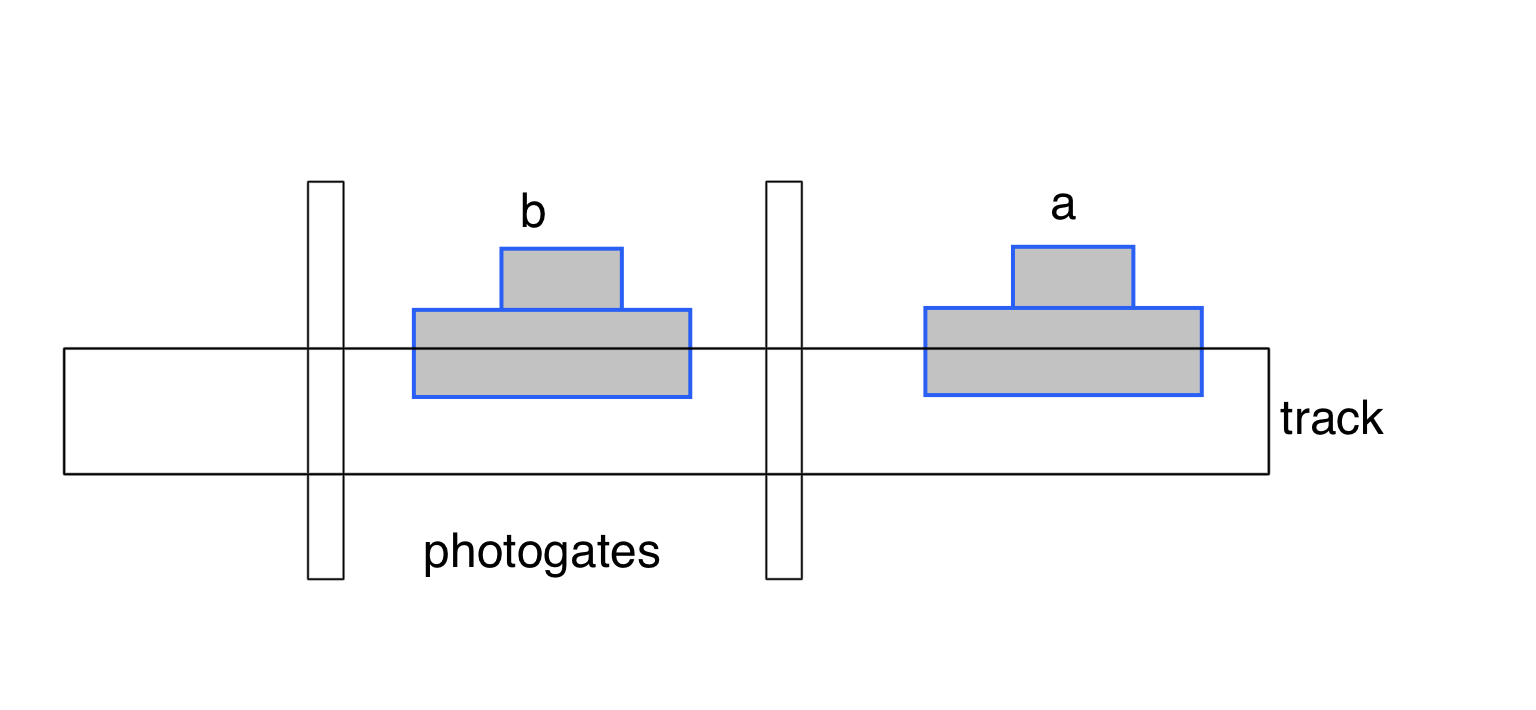
\includegraphics[width=5.5in]{./IMG_0639.PNG}
\captionof{figure}{Experimental setup}
\end{center}
\section{Results}
\label{sec:org55bdcd9}

Here are our results for the inelastic case:

\begin{center}
\captionof{table}{Inelastic collision results}
\begin{tabular}{c|c|c|c|c|c}
\(m_a\) (kg) & \(m_b\) (kg) & \(v_a\) (cm/s) & \(v_f\) (cm/s) & \(\Delta p\) (kg \(\cdot\) m/s) & \(\Delta K\) (J)\\
\hline
0.2037 & 0.2028 & 24.5 & 11.6 & -0.00275\textpm{}0.00245 & -0.00338\\
0.2037 & 0.2528 & 30.7 & 21.1 & 0.0338\textpm{}0.0023 & -0.000139\\
0.2037 & 0.3028 & 25.5 & 16 & 0.0291\textpm{}0.0030 & -0.0000563\\
\end{tabular}
\end{center}

Here are our results for the elastic case:

\begin{center}
\captionof{table}{Elastic collision results}
\begin{tabular}{c|c|c|c|c|c|c}
\(m_a\) (kg) & \(m_b\) (kg) & \(v_{a,i}\) (cm/s) & \(v_{a,f}\) (cm/s) & \(v_{b,f}\) (cm/s) & \(\Delta p\) (kg \(\cdot\) m/s) & \(\Delta K\) (J)\\
\hline
0.2042 & 0.2025 & 60.2 & -13.3 & 43.6 & -0.0400\textpm{}0.0106 & -0.0159\\
0.2042 & 0.2526 & 55.2 & -4.3 & 44.8 & -0.00833\textpm{}0.00084 & -0.005573\\
0.2042 & 0.3026 & 51 & -7.7 & 40 & -0.0188\textpm{}0.0008 & -0.00174\\
\end{tabular}
\end{center}
\section{Discussion}
\label{sec:org52fb8de}

The overall amount of momentum lost in our experiments are small. However, the amount of overall momentum in the system is small: our largest initial momentum was in the first trial of the elastic collision, and that only had 0.11 kg\(\cdot\)m/s of momentum.

Using \(\frac{\Delta p}{p_i}\) and \(\frac{\Delta K}{K_i}\) on our trials yields the following table of loss in our trials:

\begin{table}[htbp]
\caption{\label{fig:diff}Percentage Difference}
\centering
\begin{tabular}{c|c|c}
Trial & \(\Delta p/p_i\) & \(\Delta K/K_i\)\\
\hline
1 & -0.0552 & -0.553\\
2 & 0.560 & -0.0211\\
3 & 0.0540 & 0.0586\\
4 & -0.503 & -0.431\\
5 & -0.0739 & -0.179\\
6 & 0.0113 & -0.0656\\
\end{tabular}
\end{table}

Some trials have a small amount of loss, at 1\%, while others approach nearly 55\%. There is no consistency.

There are two possible sources of error in this lab: ensuring \(v_{b,i}\) is zero, and ensuring there are no net external forces. Ensuring \(v_{b,i}\) is zero is tricky because of the nature of the setup: since the guide reduces friction to basically zero, \emph{any} small push on glider \(b\) gives it some momentum, including the force of lifting a finger off glider \(b\). As such, it was extremely difficult to make sure glider \(b\) had no momentum prior to the collision.

Additionally, we observed that the gliders, when left stationary, would begin to slide towards one direction over time. This means there is a slight net external force from gravity, pulling it down to the side of the ramp angled slightly downwards.

Further experimentation is required to account for this error. A future experiment might include assuming \(v_{b,i}\) is not zero by pushing both gliders into each other and having them collide between the photogates, rather than having glider \(b\) be stationary in between both photogates.

For our error propagation, since we used very precise instruments with minimal human input, we had very small error propagation. However, we did not properly account for the error of \(v_{b,i}\) not being zero. In our calculation, we assumed that there were two main sources of error: error from measuring the velocity of glider \(a\) before the collision, which is also equal to the error from measuring the velocity of glider \(a\) and glider \(b\) after the collision, and error from measuring the mass of the gliders. This does not account for glider \(b\) having a non-zero initial velocity, since Equations \ref{eq:inelastic} and \ref{eq:elastic} have no \(v_{b,i}\) component.
\section{Sample Calculations}
\label{sec:orgff02e7b}

We used a spreadsheet for all of our calculations.

The following is for the inelastic case:

For calculating \(\Delta p\), we used \texttt{=(A2+B2)*D2/100-A2*C2/100}. For calculating \(\Delta K\), we used \texttt{=1/2*(A2+B2)*(D2/100)\textasciicircum{}2-1/2*A2*(C2/100)\textasciicircum{}2}. For calculating the values obtained in Table \ref{fig:diff}, we used \texttt{=E2/(A2*C2/100)} and \texttt{=F2/(1/2*A2*(C2/100)\textasciicircum{}2)} respectively. Our error propagation squared was
\begin{verbatim}
=(-A2)^2*B13^2+(D2-C2)^2*E13^2+(A2+B2)^2*B13^2+D2^2*E13^2~
\end{verbatim}
and doing \texttt{=sqrt(A18)} yielded our error.

This is the spreadsheet for the inelastic case:

\begin{center}
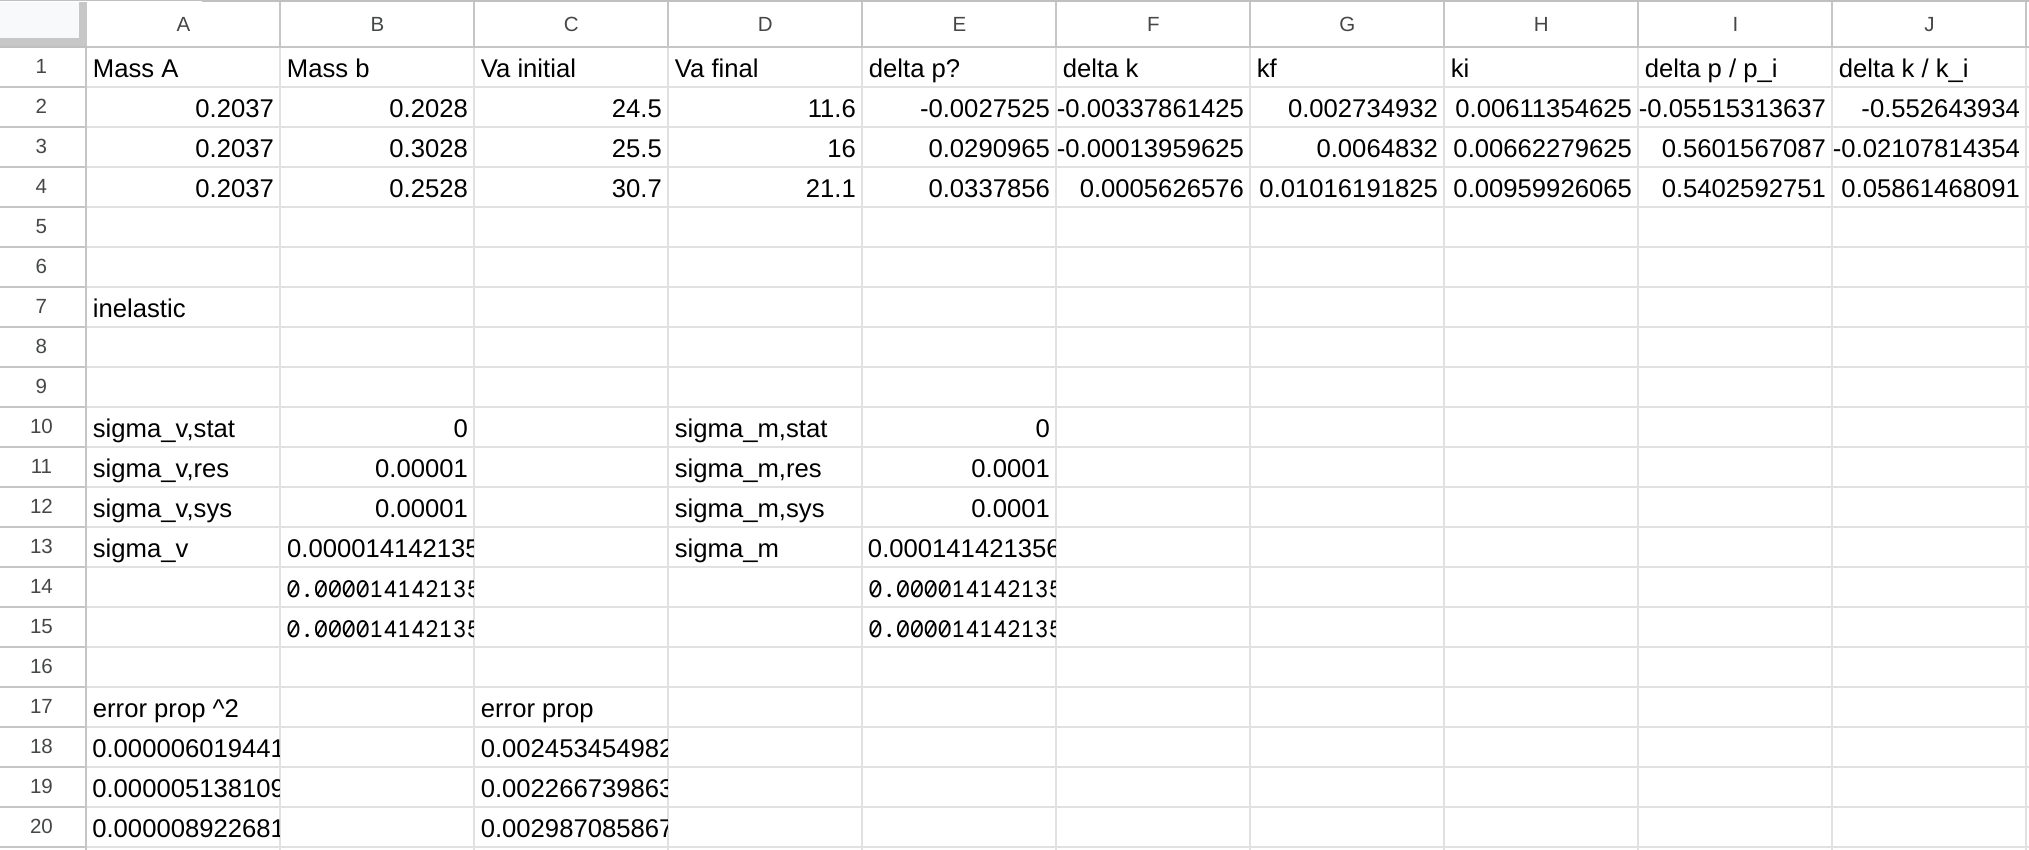
\includegraphics[width=6.5in]{./inelastic.png}
\end{center}

The following is for the elastic case:

For calculating \(\Delta p\), we used \texttt{=M2*(P2/100-O2/100)+\$N\$2*Q2/100}. For calculating \(\Delta K\), we used \texttt{=1/2*M2*((P2/100)\textasciicircum{}2-(O2/100)\textasciicircum{}2)+1/2*N2*(Q2/100)\textasciicircum{}2}. For calculating the values obtained in Table \ref{fig:diff}, we used \texttt{=R2/(M2*O2/100)} and \texttt{=S2/(1/2*M2*(O2/100)\textasciicircum{}2)} respectively. Our error propagation squared was
\begin{verbatim}
=(P2-O2)^2*E13^2+P2^2*E13^2+(-M2)^2*B13^2+M2^2*B13^2+N2^2*B13^2
\end{verbatim}
and doing \texttt{=sqrt(M18)} yielded our error.

This is the spreadsheet for the elastic case:

\begin{center}
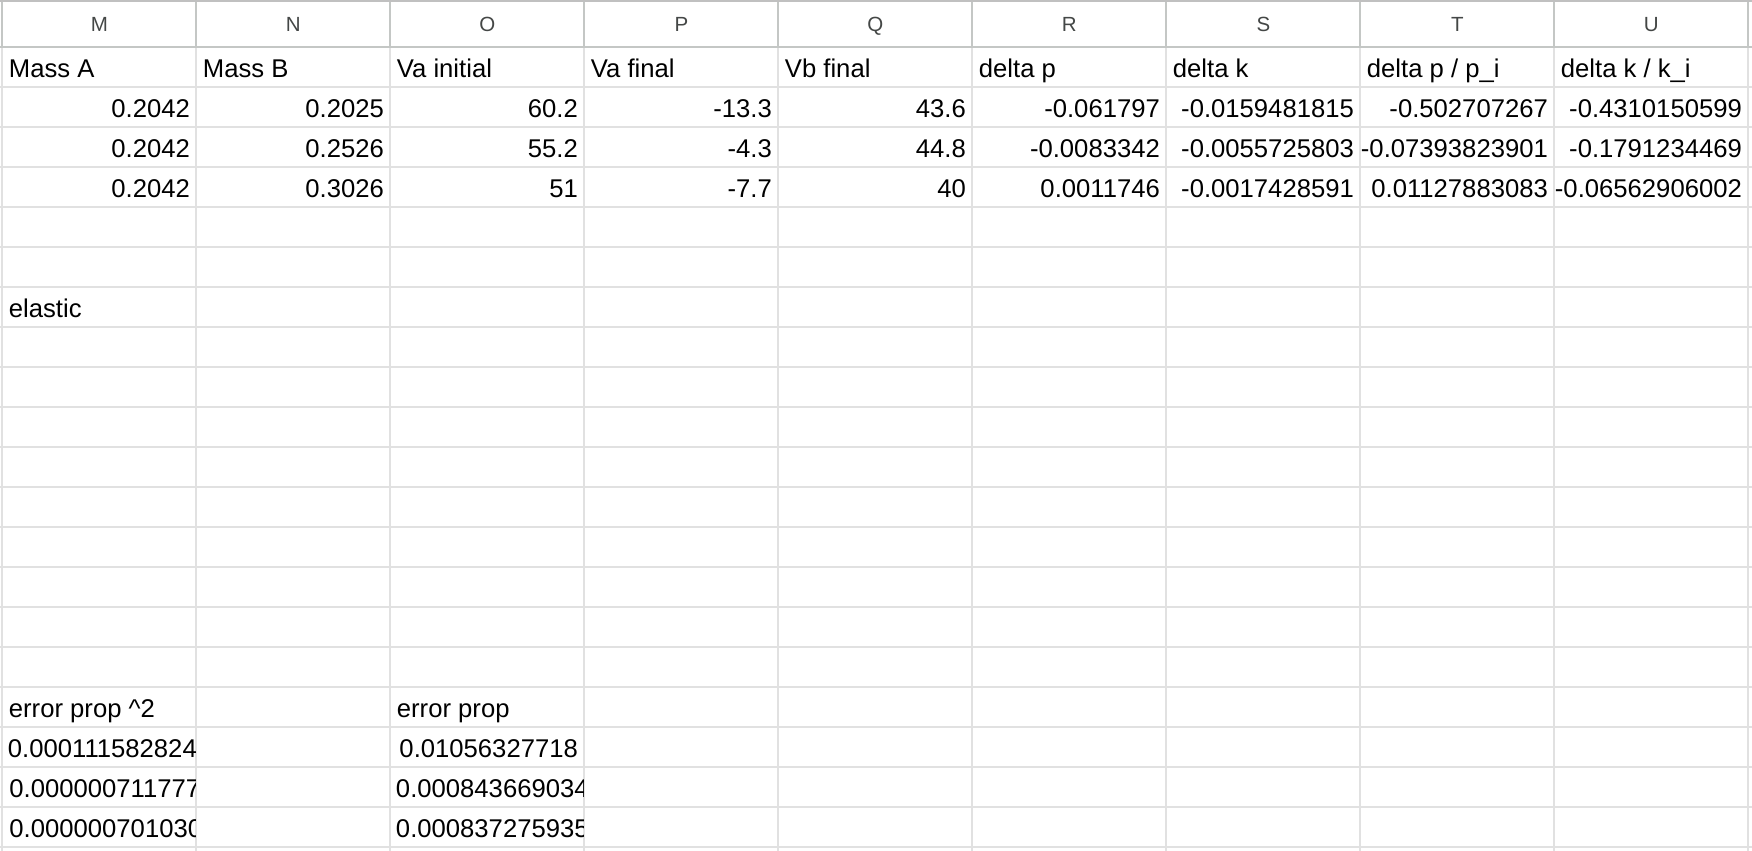
\includegraphics[width=6.5in]{./elastic.png}
\end{center}
\end{document}
